% !TeX spellcheck = it_IT

\documentclass[twoside,italian]{book}
\usepackage[T1]{fontenc}
\usepackage[utf8]{inputenc}
\usepackage{titling}
\setcounter{secnumdepth}{3}
\setcounter{tocdepth}{3}
\usepackage{babel}
\usepackage{gensymb}
\usepackage{tcolorbox}
\usepackage{listings}
\usepackage{xcolor}

\usepackage[colorlinks = true, urlcolor=blue]{hyperref}
\usepackage[a4paper,top=2.5cm,bottom=2cm,left=2cm,right=2cm]{geometry}
\usepackage{colortbl}
\usepackage{tabu}
\taburulecolor{black}
\usepackage{sectsty}
\chapterfont{\flushright}
\graphicspath{{"images/"},{.}}

\newcommand{\nlinea}{
	\leavevmode
	\\
}

\definecolor{default}{rgb}{0,0,0} % usato per il testo
\definecolor{code}{rgb}{0.19, 0.55, 0.91} %usato per il tag code
\definecolor{lred}{rgb}{1,0.3,0.3} %per le tabelle
\definecolor{codeback}{rgb}{0,0,0} %lst background
\definecolor{codefore}{rgb}{0,1,0} % lst testo
\definecolor{fsuggerimento}{rgb}{0.01,0.85,0.77} %colore testo titolo suggerimento
\definecolor{bsuggerimento}{rgb}{0.38,0,0.93} %colore testo sfondo suggerimento


\lstdefinestyle{mystyle}{
	backgroundcolor=\color{codeback},
	basicstyle=\ttfamily\color{codefore} %TODO FIX bisogna riprendere il colore precedente
}

\newcommand{\centcode}[1]{
	
	\definecolor{centcode}{rgb}{0.5,0.1,0.1}
	
	\begin{center}
	 	\texttt{\textcolor{centcode}{#1}}
	\end{center}
	
	
}

\newcommand{\code}[1]{
	\texttt{\textcolor{code}{#1}}
}

\lstset{
	style=mystyle,
	breaklines,
	frame=shadowbox,
	rulesepcolor=\color{gray},
	framexleftmargin=3mm,
	inputencoding=utf8,
	extendedchars,
	literate={à}{{\'a}}1,
	alsoletter={.}
}

\begin{document}
	
	\pretitle{%
		\begin{center}
			\LARGE
			
\includegraphics[width=\linewidth]{arch-wallpaper.png}\\[\bigskipamount]
		}
		\posttitle{\end{center}}
	
	\begin{titlepage}
		
		
		
		\title{Guida Installazione Arch}
		
		\author{by PsykeDady}
		
		\date{AAAA-MM-DD}
		
	\end{titlepage}

	\maketitle
	\hypersetup{colorlinks=true, linkcolor=black}

	\newpage{}
	
	
	
	\begin{LARGE}
		\textbf{
			Prefazione: a chi è indirizzata questa guida?
		}


	\end{LARGE}

	\color{default}
	\nlinea
	questa guida si prefigge lo scopo di essere generale un po' orientata a chiunque si avvicini la prima volta nel mondo di Archlinux. Tuttavia è stata seguita seguendo le mie esigenze e le mie esperienze acquisite nel campo. Al tempo in cui sto scrivendo questa prefazione (estate 2018) ho alle spalle soli 3 anni di abilità acquisite su archlinux, installando tuttavia più e più volte la distribuzione su vari calcolatori (pc fissi, portatili, macbook etc..)
	\nlinea \nlinea
	Se c'è comunque una consapevolezza di cui il tempo, le mie e le esperienze altrui mi hanno fatto dono è che, inevitabilmente, \textbf{ogni calcolatore gode di un esperienza unica in termini di prestazioni, estetica e praticità della configurazione distribuzione/kernel/parametri installati da colui che si appresta ad utilizzarci GNU/Linux sopra}. Questa affermazione, se pur posso assicurare abbia un alto grado di verità, tende ad entrare difficilmente nelle mentalità di chi da tempo, ormai, tende ad avere atteggiamenti da stadio anche nei confronti della più assoluta libertà che dovrebbe invece professare la community di Linux.
	\nlinea \nlinea
	Inoltre consiglio a \textbf{tutti} coloro che si avventurano nella piccola impresa di installare archlinux, di tenere sempre sottomano la guida \textit{ultima} di tutti noi arch-user (e non solo), la \href{https://wiki.archlinux.org/index.php/Installation_guide}{wiki}: un'enorme fonte di conoscenza sul mondo linux che risolve problemi in qualsiasi ambito, o quanto meno vi aiuta a risolverli indirettamente. Tutto ciò che troverete in questa guida altro non è che un estratto di piccole sezioni della wiki che io uso sempre per installare archlinux. La guida è inoltre disponibile in moltissime lingue, tra cui l'italiano.
	\nlinea \nlinea
	Ricordo inoltre che per chi volesse provare un Archlinux con installer user-friendly, esiste \href{https://antergos.com/}{Antergos}, una distro su base arch completamente personalizzabile al momento dell'installazione, molto ma molto user-friendly.
	\nlinea
	Rimane comunque consigliato, a mio avviso, non scegliere archlinux come distribuzione per approcciarsi la prima volta con il mondo GNU/Linux, ma scegliere distro più "alla mano" come \textbf{Ubuntu}, \textbf{Fedora}, \textbf{Linux Mint} o \textbf{Deepin}.
	\nlinea \nlinea
	Un ultima considerazione: questo file è in continuo aggiornamento, motivo per il quale la data, in pagina principale, non è ancora specificata.
	Detto questo: buon divertimento e benvenuti nel fantastico mondo di Archlinux

	\begin{figure}[h!]
		\flushright
		
\includegraphics[width=0.25\textwidth] {archlogo.png}
	\end{figure}



		\begin{flushright}
			\vspace*{\fill}{
				\textit{...Linux è sinonimo di libertà e rispetto...}
			}
		\end{flushright}


	\newpage{}

	\tableofcontents

	\flushleft
	\chapter {Preparare il supporto di installazione }



		\section{Metodo 1 da Linux : dd}

			Il primo semplice metodo consiste del preparare la pennina con il famoso tool \textit{dd}:

			\centcode{\# dd if=/percorso/iso of=/dev/sdX bs=4M status=progress}

			sostituire a X la lettera del mezzo di installazione, inserire la pennina e digitare \code{\# fdisk -l} e quindi leggere l'output fino ad arrivare a quella che sembra essere la vostra pennina, leggendone le coordinate

			in seguito all'installazione, per poter riutilizzare la pennina nuovamente, dovrete azzerarla con lo stesso tool:
			\centcode{\# dd if=/dev/zero of=/dev/sdXY bs=4M status=progress}

			\begin{tcolorbox}[floatplacement=b,width=\textwidth,colback={blue},title={NOTA BENE:},colbacktitle=gray,coltitle=white,colupper=white]
				un uso intensivo di dd potrebbe rovinare la pennina, in quanto ne sovrascrive il contenuto bit a bit. Fare quindi attenzione, meglio utilizzare pennine a basso costo e soprattutto non molto capienti
			\end{tcolorbox}

		\section{Metodo 2  da Linux:  copia su fat32 (Consigliato UEFI)}
			un altro metodo consiste nel copiare il contenuto della ISO in un file system FAT32, questo metodo presenta diversi vantaggi, ma funziona solo con macchine UEFI

			creare quindi due directory dove montare la ISO e la USB di installazione:
			\centcode{mkdir \{usb,iso\}}

			montare la iso utilizzando: \centcode{\# mount -o loop /percorso/iso iso}

			se non lo si è ancora fatto, formattare la pennetta in fat32, supposto sia /dev/sdX il percorso della pennina, seguire queste istruzioni per formattarne il contenuto (effettuare le operazioni si \textbf{su} o con \textbf{sudo}):\\


\begin{lstlisting}
		dd if=/dev/zero of=/dev/sdX #da eseguire solo se si vuole completamente resettare la pennina

		fdisk /dev/sdX #si entrera' in modalità fdisk, scrivere e premere invio i prossimi comandi
		o
		p
		1
		2048
		#(invio senza scrivere nulla oppure scegliere una dimensione)
		t
		b
		w #si uscira' dalla modalita' fdisk

		#e' possibile alternativamente a fdisk, usare cfdisk che e' piu' user-friendly

		mkfs.fat /devX1

		mount /dev/sdX1 usb

		dosfslabel /dev/sdX1 ARCH_AAAAMM  #sostituendo ad AAAA ed MM le stesse date che trovate sulla iso
\end{lstlisting}



			In questo momento, si ha nelle cartelle usb e iso, montati rispettivamente la usb e il contenuto della iso. Ci apprestiamo dunque a copiare il contenuto della iso nella usb

			\centcode{cp -r iso/* usb}

			Consiglio a questo punto di sincronizzare  i dischi e smontare le cartelle, per evitare che le modifiche non vengano attuate correttamente:

\begin{lstlisting}
		sync
		umount  {usb,iso}
\end{lstlisting}



			La pennina è pronta per i sistemi UEFI. Questo metodo è più sicuro di dd ma funziona su meno sistemi, eventualmente si può pensare di usare syslinux per ampliare ulteriormente il bacino di pc che vedranno la pennetta come avviabile, scaricare quindi dal proprio gestore di pacchetti l'ultima versione di \textbf{syslinux} e di \textbf{parted} ed eseguire i prossimi comandi (prima di smontare la usb):

\nlinea
\begin{lstlisting}
		extlinux --install usb/arch/boot/syslinux
		dd bs=440 conv=notrunc count=1 if=/usr/lib/syslinux/bios/mbr.bin of=/dev/sdX
		parted /dev/sdX toggle 1 boot
\end{lstlisting}



			\begin{tcolorbox}[floatplacement=b,width=\textwidth,colback={white},title={ATTENZIONE:},colbacktitle=red,coltitle=white,colupper=red]

				quest'ultimo passo non l'ho mai applicato personalmente, ma l'ho letto sulla wiki e ve l'ho voluto riportare. Se qualcosa non dovesse funzionare, vi invito  a documentarvene personalmente dalla guida ufficiale

			\end{tcolorbox}


		\section{Metodo 3 da Linux : varie GUI}
			Se non amate molto sporcarvi personalmente le mani durante queste operazioni sono disponibili moltissimi programmi che lo fanno per voi. Personalmente (ma anche la guida ufficiale) sconsiglio fortemente l'utilizzo del noto programma \textbf{uNETbootin}, in quanto tende a funzionare solo con ubuntu e derivate. Comunque sia elencherò una serie di software che ho usato io e che \textit{spesso} funzionano:

			\begin{itemize}
				\item etcher
				\item suse image writer
				\item deepin usb maker
				\item Fedora media writer
			\end{itemize}


		\section{Altri S.O.}

			Su sistemi operativi OSX consiglio di usare \textbf{l'utility Disco} di sistema.
			\\
			Su sistemi operativi Windows invece consiglio l'uso di \textbf{Rufus} o \textbf{LiLi USB} (meno consigliato su sistemi UEFI comunque).
			Se vi doveste trovare male con i primi, altri utenti archlinux mi hanno consigliato i seguenti programmi:
			\begin{itemize}
				\item Win32DiskImager
				\item USBWriter
			\end{itemize}


	\chapter{Hello world, i'm Archlinux! Nice to meet you}

		Supponendo ora che siate riusciti da soli ad avviare il supporto attraverso le impostazioni del vostro BIOS o le impostazioni EFI del vostro sistema, o che ancora l'abbiate avviata attraverso virtualbox e che vogliate farvi una VM con sopra archlinux, possiamo quindi passare alle prime fasi dell'installazione.

		Avviando arch, se tutto va bene, dovreste ritrovarvi davanti ad una schermata simile:

		\begin{figure}[h!]
			\centering
			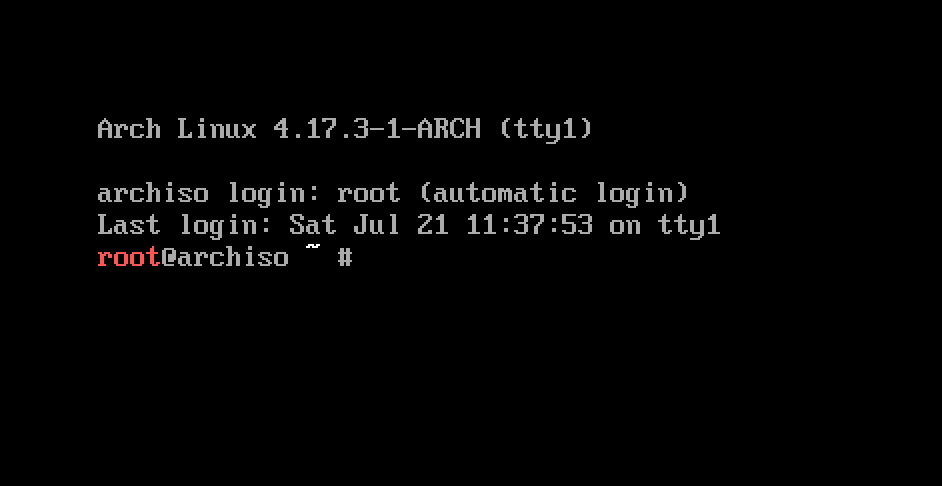
\includegraphics[width=0.75\linewidth] {prima_schermata.png}
			\caption{ecco a voi la schermata da cui tutto avrà inizio...}
		\end{figure}

		L'utente un po' inesperto o pratico solo di installazioni Ubuntu/OSX/Windows sarà spaesato, ma nessuna paura, è tutto molto più semplice di ciò che si pensa.

		Ma prima di tutto, se avete una tastiera italiana, digitate: \centcode{loadkeys it} 
		\nlinea
		se avete uno schermo hidpi digitate anche:
		\centcode{setfont /usr/share/kbd/consolefonts/sun12x22.psfu.gz}
		\nlinea
		così vedrete meno madonnine volare in cielo...
		
		\begin{tcolorbox}[floatplacement=b,width=\textwidth,colback={blue},title={NOTA BENE:},colbacktitle=gray,coltitle=white,colupper=white]
			nella cartella \code{/usr/share/kbd/consolefonts/} trovate molti altri font, scegliete solo quelli 12x22 per la leggibilità massima
		\end{tcolorbox}
		
		

		\section{preparazione del disco di installazione}

			La prima cosa da fare è preparare il disco di installazione, attraverso i comandi \code{blkid} o \code{fdisk -l} scopriamo quindi le coordinate del nostro disco ed eventualmente della partizione se preparata in anticipo attraverso altri sistemi operativi (può essere utile spesso preparare tutto attraverso una live di ubuntu con gparted se si è alle prime armi e si hanno dati da preservare).\\

			Ci vuole comunque un po' di organizzazione, bisogna sapere in anticipo in quante partizioni si vuole suddividere la propria installazione, se si è su un sistema UEFI, se si hanno più dischi e se si hanno altre installazioni da preservare.\\

			La guida supporrà che il disco sia inizialmente non inizializzato, sia l'unico disco e che non si hanno altri sistemi operativi presenti. Supporrò inoltre di voler suddividere l'installazione in: root, home e swap. Un altra condizione supposta sarà quella di avere un sistema EFI con tutto quello che ne deriva.\\
			
					
			\begin{tcolorbox}[floatplacement=b,width=\textwidth,colback=fsuggerimento,colbacktitle=bsuggerimento,coltitle=fsuggerimento, colupper=bsuggerimento,title={SUGGERIMENTO}]
				 Lo spazio di Swap è uno spazio utilizzato dal sistema per sopperire alla mancanza di memoria RAM sufficente a far funzionare correttamente tutti i programmi. In genere si usa riservarne spazio uguale alla RAM per usufruire anche della funzione di ibernazione, che consente di spegnere il computer senza perdere la sessione di lavoro corrente (diversamente dalla sospensione non consuma batteria). Per pc con RAM maggiore di 4Gb non consiglio di usare la swap a meno di usare anche l'ibernazione, un alternativa può essere anche quella di usare il \textbf{file di swap} anziché la partizione. Maggiori informazioni si troveranno nella sezione che riguarda le configurazioni di sistema.
			\end{tcolorbox}


			Abbiamo quindi il nostro disco su \textbf{/dev/sda}, vuoto e non inizializzato in alcun modo (un disco vergine per intenderci, come quello che potremmo trovarci in una macchina virtuale). Alternativamente si può pensare che abbiamo un disco  di cui il contenuto non ci interessa, quindi le seguenti operazioni lo formatteranno completamente: \centcode{gdisk /dev/sda}
			in questo modo si entrerà in modalità gdisk, che installerà uno schema di partizioni di tipo GPT. se non si ha a che fare con UEFI, è consigliato usare \code{fdisk} o \code{cfdisk}, e avere a che fare con schema di partizioni tradizionale.\\
			Come per \textit{fdisk} e \textit{cfdisk}, anche \textbf{gdisk} ha un alternativa user-friendly che è \textbf{cgdisk}. Prendetela in considerazione se non volete seguire le istruzioni che seguiranno ma avere accesso ad un interfaccia più pratica.
			Se avete scelto per \code{gdisk}, premere quindi in sequenza:\\

\begin{lstlisting}
	o
	n
	1
	(invio senza scrivere niente)
	+200M
	ef00

	n
	2
	(invio senza scrivere niente)
	+XXXG
	# (sostituendo a XXX il numero di Giga che volete dare alla vostra root)
	(invio senza scrivere niente)

	n
	3
	(invio senza scrivere niente)
	+YYYG
	#sostituendo a YYY il numero di Giga che volete dare alla home, in genere qua si mette la maggiorparte dello spazio
	(invio senza scrivere niente)

	n
	4
	(invio senza scrivere niente)
	+ZZG
	#sostituendo a ZZ il numero di Giga che volete dare alla  swap.
	8200

	w
\end{lstlisting}



			dopo essere usciti dalla modalità gdisk, possiamo accertarci della situazione usando il comando: \code{gdisk -l} oppure con \code{blkid}.
			Per usare le partizioni comunque è necessario formattarle\\


\begin{lstlisting}
	mkfs.fat /dev/sda1
	mkfs.ext4 /dev/sda2
	mkfs.ext4 /dev/sda3
	mkswap /dev/sda4
\end{lstlisting}



			dunque possiamo iniziare a montarle:


\begin{lstlisting}
	mount /dev/sda2 /mnt
	mkdir -p /mnt/boot/efi
	mkdir /mnt/home
	mount /dev/sda1 /mnt/boot/efi
	mount /dev/sda3 /mnt/home
	swapon /dev/sda4
\end{lstlisting}



			La sezione riguardante la configurazione dei dischi finisce qua.

		\section{Installazione dei pacchetti e connessione al mondo esterno}

			Stop. senza internet non si va da nessuna parte.\\

			Se quindi siete connessi via cavo, basta dare \code{dhcpcd}, altrimenti archlinux fornisce una comodissima interfaccia di rete wireless, a cui potete accedere così: \centcode{
				wifi-menu
			} Scegliete quindi il vostro SSID di fiducia, scrivete la password (se ne avete una) e date \code{dhcpcd} per forzare il router a rilasciarvi un indirizzo ip. Ben fatto, siete connessi! Sicuri? Per accertarcene possiamo dare \centcode{ping -c 3 www.google.com} se tutto va bene, vi risponderà che son stati trasmessi e ricevuti 3 pacchetti. Ora che siamo sicuri possiamo andare avanti.\\

			Arch offre un modo davvero comodo di installare i pacchetti iniziali sulle nuove installazioni, attraverso lo script \textbf{pacstrap}:\\
			\centcode{pacstrap /mnt base base-devel net-tools dialog netctl wpa\_supplicant grub efibootmgr}

			se tutto va per il meglio (spero per voi) il vostro /mnt sarà adesso abbastanza popolato.

		\section{prime configurazioni}
			creiamo quindi il vostro fstab che permetterà di montare le cartelle nel giusto ordine all'avvio:
			\centcode{genfstab -pU /mnt >> /mnt/etc/fstab}

			ed entriamo quindi in chroot attraverso un comodissimo script arch:
			\centcode{arch-chroot /mnt}

			settiamo la password di root: \centcode{passwd}
			e modifichiamo il file fstab creato in precedenza sostituendo nella riga della swap, il parametro \textit{none} scrivendo \textbf{swap}

			configuriamo quindi il grub: \centcode{
			grub-mkconfig -o /boot/grub/grub.cfg \\
			grub-install /dev/sda
			}

			possiamo quindi dare un nome alla nostra macchina in rete:\centcode{echo "NOMEPC" > /etc/hostname}

			Impostiamo quindi la lingua: andando ad editare (con \code{nano}, \code{vi} o qualunque altro editor ci piace usare) il file \textit{/etc/locale.gen} decommentando le tre linee che iniziano con \textbf{it\_IT}, successivamente diamo il comando \centcode{locale-gen}

			successivamente generiamo un buon \textit{/etc/locale.conf}, usiamo il nostro editor di testo preferito e scriviamo:

\begin{lstlisting}
	LANG=it_IT.UTF-8
	LC_COLLATE="C"
	LC_TIME="it_IT.UTF-8"
	LANGUAGE="it_IT:en_GB:en"
\end{lstlisting}

			impostiamo la lingua del tty con:
			\centcode{echo "KEYMAP=it" > /etc/vconsole.conf}

			e impostiamo il fuso orario di sistema con:
			\centcode{ln -sf /usr/share/zoneinfo/Europe/Rome /etc/localtime}

		\section {programma di installazione terminato}

			Il sistema è installato correttamente, adesso andiamo per smontare le partizioni:
\begin{lstlisting}
	exit
	umount /mnt/boot/efi
	umount /mnt/home
	umount /mnt
	swapoff
	sync
	poweroff # o reboot per riavviare
\end{lstlisting}

			possiamo quindi riavviare e continuare con le configurazioni tramite l'utente root e non in ambiente di chroot

	\chapter{Configurazioni di sistema}

		Dopo aver riavviato e tolto la chiavetta, dovremmo trovare la possibilità di avviare archlinux tramite grub, se così non fosse reinserite la chiavetta, rimontate le partizioni e rifate il chroot, cercando la soluzione al problema tramite la guida wiki.
		Da qui in poi sarà supposto che voi abbiate il sistema funzionante e possiate fare il login tramite account di root.

		Inserite quindi come nome \textit{root} e come password quella impostata durante le configurazioni precedenti. È quindi tempo di fare un po' di configurazioni a sistema appena installato!

		\section{Connettiamoci al mondo esterno e alcuni consigli iniziali}

			Come sempre la prima cosa da fare è connettersi. lo si può fare esattamente come prima tramite \code{dhcpcd} e nel caso di una wifi \code{wifi-menu}.

			Il primo consiglio che innanzitutto do è quello di eseguire subito un upgrade del sistema e dei repository:\centcode{pacman -Syu}
			Consiglio poi di installare alcuni pacchetti che nel 90\% dei casi vi saranno utili\centcode{pacman -S linux-headers os-prober git bash-completion}Nello specifico, os-prober vi serve nel caso in cui pianificate ( o abbiate ) una macchina con più sistemi operativi installati.

		\section{Server e driver}

			In ambienti linux, senza motore grafico, possiamo usare il pc al più come server. Oggi giorno la produttività dipende strettamente da ciò che vediamo e come interagiamo. Per questo motivo installiamo il server grafico, oggi Xorg, nonostante ci siano valide alternative, risulta ancora la realtà più consolidata, vi consiglio dunque di installarlo a prescindere da ciò che poi proverete. Insieme a Xorg, è consigliato installare il suo sistema di init, utile nel caso in cui non vogliate un DM o il vostro non funzioni a dovere. Quindi:\centcode{pacman -S xorg-server xorg-xinit}
			Potete quindi impostare nel file \textit{$\sim$/xinitrc} il comando per utilizzare  il vostro DE preferito (quando ne avrete uno).

			Installare i driver è anche abbastanza semplice, se avete installato arch su una macchina virtuale virtualbox, vi basterà digitare: \centcode{pacman -S virtualbox-guest-utils}altrimenti andiamo ad identificare la vostra scheda video con \code{lspci} \centcode{lspci | grep VGA}l'output riporterà al suo interno: \textbf{intel}, \textit{ati} o \textit{nvidia}. In base a cosa riporta andiamo ad installare i driver \textit{open} relativi:
\begin{lstlisting}
	#per installare i driver intel
	pacman -S xf86-video-intel

	#per i driver ati
	pacman -S xf86-video-ati

	#per nvidia
	pacman -S xf86-video-nouveau
\end{lstlisting}

			per installare i driver proprietari vi invito invece a visitare la wiki relativa.
			
			Alcune volte può essere necessario installare i vecchi driver synaptics per il touchpad, tanto meglio nel caso averli già pronti:
			\centcode{pacman -S xf86-input-synaptics}

		\section{Aggiunta utente, creazione cartelle utente e cifratura home }

			È sempre bene utilizzare l'account root solo se strettamente necessario, altrimenti è meglio impostare un utente amministratore o semplice (ancora meglio).

			per aggiunta di un utente amministratore digitare:
			\centcode{useradd -m -g users -G wheel,video,audio,sys,lp,storage,scanner,games,network,disk,input -s /bin/bash <nome utente>}

			per un amministratore non utente basta eliminare il gruppo \textbf{wheel} dal codice precedente.\\
			Impostiamo quindi una password per l'utente appena creato: \centcode{passwd <nome utente>}e indichiamo al programma sudo ( che ci permette di effettuare operazioni in modalità amministratore) tramite \textit{visudo}:

\begin{lstlisting}
	#impostiamo prima un editor di testo a noi piu' amichevole, di default e' vi
	export EDITOR=<nome editor>
	visudo
\end{lstlisting}

			a questo punto esistono due modi di impostare i permessi di amministratore, con richiesta della password (consigliato) e senza richiesta.

			nel primo caso decommentare la riga:\centcode{wheel ALL=(ALL) ALL}
			nel secondo decommentare: \centcode{wheel ALL=(ALL) NOPASSWD: ALL}

			A questo punto configuriamo le cartelle utente, installiamo \centcode{pacman -S xdg-user-dirs}. Al nostro accesso con l'utente digitiamo \centcode{xdg-user-dirs-update} e ci dovremmo trovare nella home tutte le cartelle utente. Nel caso non siano in italiano si può editare il file \textit{/home/<nome utente>/.config/user-dirs.dirs} inserendo ad uno ad uno i nomi che desideriamo sostituire.
			\nlinea 

			\nlinea

			\hrule
			\nlinea

			\nlinea

			\textbf{Il prossimo step è opzionale, se non volete eseguirlo passate direttamente alla prossima sezione:} potete decidere di cifrare il contenuto della vostra home, un po' come succede nei telefoni che possiedono metodo di sblocco con impronta digitale. Per farlo la prima cosa è installare alcuni pacchetti \centcode{pacman -S ecryptfs-utils keyutils rsync lsof}
			Quindi caricare l'apposito modulo del kernel:\centcode{modprobe ecryptfs}. Potrebbe essere necessario apportare una modifica al file \textit{/etc/mkinitcpio.conf} e scriverci all'interno, nella sezione \textbf{MODULES}, il nome del modulo per forzarne il caricamento ad ogni avvio del pc. Successivamente ricompilare il servizio di avvio \centcode{mkinitpcio -p linux}Usare quindi il tool per la migrazione della home, per avviare questa fase è necessario che voi non abbiate alcun processo aperto con l'utente di cui volete cifrare la home: \centcode{ecryptfs-migrate-home -u <nome utente>}
			Seguire le istruzioni indicate. Per completare la procedura, uscite dal vostro account root con \code{exit} ed entrate con quello dell'utente. Verificate quindi con \code{ls} che siano state criptate tutte le cartelle (dovrebbe apparire Access-your-data.desktop e un altro file di testo)

			Quindi  decriptate e ri-criptate voi stessi la home usando i due tool \centcode{
				ecryptfs-mount-private \#per decriptare\\
				ecryptfs-umount-private \#per ricriptare
			}
		
			Potete usare i due comandi ogni volta che volete cifrare o decifrare la cartella home manualmente, può accadere alle volte che la cifratura non avvenga per processi aperti su file all'interno della home. Si può quindi forzare il procedimento con questo comando \centcode{umount.ecryptfs\_private}

			uscite dall'account user (dopo aver smontato la cartella) e rientrate con root per maggiore comodità.
			\nlinea
			\nlinea
			Ora è necessario ( a meno che non vogliate farlo a mano ogni accesso) impostare l'auto-mounting della home criptata all'accesso.
			Facciamo un backup del file \textit{/etc/pam.d/system-auth} \centcode{cp /etc/pam.d/system-auth /etc/pam.d/system-auth.old}e apriamo \textit{/etc/pam.d/system-auth} con il nostro editor preferito.\\
			Da adesso facciamo \textbf{MOLTA} attenzione, sbagliando qualunque cosa potremmo non poter più accedere a nessun account (a meno di aggiustare poi le cose con l'iso di arch), andiamo ad aggiungere dopo la stringa che contiene \textbf{auth required pam\_unix.so} la seguente linea:
			\centcode{auth    required    pam\_ecryptfs.so unwrap}

			Dopo la linea linea che contiene \textbf{password required pam\_unix.so} aggiungiamo: \centcode{password    optional    pam\_ecryptfs.so}

			E infine dopo la linea che contiene \textbf{session required pam\_unix.so} aggiungiamo:\centcode{session required pam\_ecryptfs.so unwrap}
			Usciamo dall'editor salvando. Per essere sicuri di aver fatto le cose a modo, apriamo un altro tty (\code{ctrl-alt-f2}) e facciamo l'accesso con l'utente. Se l'accesso avviene correttamente, e se la cartella viene correttemente decriptata, allora è tutto ok. Altrimenti ritornate immediatamente nel primo tty (\code{ctrl-alt-f1})  correggete l'errore nel file o, nel caso non ci riusciate, eliminate tutte le modifiche facendo tornare il file allo stato originale attraverso il backup.
			Se tutto è andato a buon fine, ricordate di far uscire con exit l'utente. Se la cartella non viene ricriptata potreste avere problemi di accesso d'ora in poi, nel caso entrate con il tty e ricriptatela con il comando di \textit{umount}.
			Ripassate quindi al tty per continuare con l'installazione.




			\nlinea

			\nlinea

			\hrule


		\section{configurare pacman e installare pakku }

			Perché Archlinux? Perché complicarsi la vita con questa tortura che ti porta a perdere una giornata per l'installazione di un sistema operativo? Le risposte sono tante, ma la prima in assoluto è il gestore di pacchetti \textbf{pacman} e tutto ciò che ne deriva, compreso il famoso \textbf{AUR: Arch User Repository}.

			Prima di tutto, abbelliamo il nostro pacman!
			Sempre con il nostro editor preferito (a proposito, il mio è nano, vi insegnerò anche a renderlo carino) modifichiamo il file \textit{/etc/pacman.conf}: andiamo a decommentare la riga con scritto \textbf{Color} e aggiungiamo sotto \textbf{ILoveCandy}.
			Poi decommentiamo dove c'è scritto \textbf{multilib} e la riga di sotto se vogliamo abilitare il supporto alle librerie a 32 bit ( necessario per alcuni programmi).
			Se volessimo aggiungere un nuovo repository lo possiamo fare seguendo il template alla fine del file, ma difficilmente ne avrete bisogno dopo che installerete un \textbf{aur-helper}.

			Installiamone quindi uno: \textbf{pakku}!
			Per lo step successivo, è \underline{\textbf{fortemente consigliato}} l'accesso con l'utente amministratore e non con root.

\begin{lstlisting}
	git clone https://aur.archlinux.org/pakku.git
	makepkg -si
\end{lstlisting}

			\textbf{pakku} usa la stessa sintassi di \textbf{pacman}, e potete sostituirlo in tutto e per tutto al package manager, l'unica differenza sta nel fatto che cerca pacchetti anche su \textbf{AUR}, un immenso repository di pacchetti offerti dalla comunità, ci trovate davvero di tutto dentro. \textbf{Ma non va eseguito come utente amministratore (con \code{sudo} per intenderci) né come utente root.}
			Tramite pakku potete visualizzare la differenza tra versione presente e quella aggiornata del software oppure visionare e modificare il PKGBUILD, è uno strumento molto potente!
			
			Pakku è scritto in NIM, un linguaggio di programmazione ad alto livello multi piattaforma, con aspetti molto molto interessante :) se siete del settore vi consiglio di leggerne qualcosa sul web
\nlinea
	\nlinea
			La fase iniziale di installazione è terminata, consiglio a questo punto di riavviare prima di continuare.
			
			
		\section{Sincronizzare orologio di sistema e Hardware}
			
			Per sincronizzare l'orologio di sistema con quello del calcolatore si può digitare:\centcode{hwclock $--$systohc $--$utc}
			
			\begin{tcolorbox}[floatplacement=b,width=\textwidth,colback={blue},title={NOTA BENE:},colbacktitle=gray,coltitle=white,colupper=white]
				NB: il comando mi è stato suggerito dalla community di Telegram. Io personalmente non ho mai dato questo comando poichè non l'ho mai ritenuto necessario. Non posso quindi in alcun modo garantire sui risultati.				
			\end{tcolorbox}
			
		\section{tmp file system}
			
			nel nostro file system una cartella speciale, \code{/tmp}, che contiene file e cartelle temporaneamente creati dai programmi per il loro corretto funzionamento. Questa cartella viene montata da \textit{systemd} automaticamente in memoria \textbf{RAM } in modo da essere resettata ad ogni arresto del calcolatore.\\
			È comunque possibile, per quei pc che non hanno un gran quantitativo di memoria disponibile, montare la cartella nello spazio di archiviazione piuttosto che in memoria volatile
			
			\begin{tcolorbox}[floatplacement=b,width=\textwidth,colback={white},title={ATTENZIONE:},colbacktitle=red,coltitle=white,colupper=red]
				Se installate frequentemente programmi da \textbf{AUR} con un \textbf{AUR-helper} è possibile che quest'ultimo, facendo tante scritture su \code{/tmp}, vi saturi facilmente la memoria, consiglio quindi questo procedimento a tutti i pc con meno di 8 GB di RAM.
			\end{tcolorbox}
			\nlinea
			Per disabilitare il montaggio automatico basta dare:
			\centcode{\# systemctl mask tmp.mount}
			
			Bisogna comunque tener conto che disabilitando questo comportamento, il contenuto della cartella dei file temporanei \textbf{non verrà più cancellato allo spegnimento del dispositivo}.
			
			Si può ritornare al comporamento di default specificando manualmente il montaggio in \code{/etc/fstab} aggiungendo questa linea di testo al file:
			\centcode{tmpfs   /tmp         tmpfs   nodev,nosuid          0  0}
			
			Si può anche specificare una size massima per evitare che la ram venga monopolizzata dalla sola partizione di file temporanei, facendo un esempio con il limite di \code{2GB} avremmo:
			\centcode{tmpfs   /tmp         tmpfs   nodev,nosuid,size=2G          0  0}
			
			Altre interessanti informazioni su \textbf{tmpfs} si trovano sulla guida di arch.
				
			
		\section{Swappiness}
			
			Se avete installato un area di swap la vostra maggior paura sarà appunto quella che il vostro pc possa usarla senza che ce ne sia la reale necessità; non è infatti detto che il sistema operativo debba aspettare di riempire la RAM prima di usare l'area di SWAP.\\
			In ogni caso questo aspetto del sistema si può benissimo controllare attraverso la \code{swappiness}\\
			Si può impostare la swappiness temporaneamente o permanentemente, nel secondo caso basta modificare il file \code{/etc/sysctl.d/99-sysctl.conf} e scrivere:
			
			\centcode{vm.swappiness=1}
			
			Come funziona questo valore però? perchè 1 e non 0?\\
			Il valore di swappiness va da \code{0 a 100} e indica il \textbf{valore di ram libera che si desidera tenere libero prima di attivare la zona SWAP}.
			Ad esempio, normalmente il valore di swappiness è \textbf{60}, questo significa che oltre il 40\% di RAM occupata, l'area di SWAP si attiva ( non finisce tutto in swap ovviamente ma il sistema tende ad assestarsi su quel valore di RAM libera).
			Nelle versioni antecedenti a linux 3.5, un valore di swappiness \code{0} significava "\textit{usa la swap solo in caso di stretta necessità}", oggi ne disattiva invece le funzioni.\\
			Maggiori informazioni \href{https://www.kernel.org/doc/Documentation/sysctl/vm.txt}{qui} e \href{https://en.wikipedia.org/wiki/Swappiness}{qui}.
			
			
					
	\chapter{Desktop Environment, Display Manager, NetworkManager e servizi systemd}

		Premessa: ad oggi l'unico Desktop Environment che \textbf{non} mi sento di consigliare, è \textbf{GNOME}. Molti prenderanno questa come una bestemmia e chiuderanno subito la guida, fatti loro. A mio parere \textbf{GNOME} ha ancora molte mancanze che mi fanno sempre desistere dal tenerlo installato sui miei sistemi, è inoltre l'unico sistema che, appena aperto, raggiunge il Gigabyte di ram occupata ( più o meno). In ogni caso la bellissima guida wiki ha una guida per ogni singolo DE che vogliate installare (e installare \textbf{GNOME} completo è davvero cosa di due comandi).\\
		La qui presente guida invece vi insegnerà a installare \textbf{Plasma}, un DE molto avanzato con consumi ram/cpu nella media.\\ Per sistemi poco prestanti consiglio \textbf{XFCE}, \textbf{LXDE} o \textbf{I3WM}, che sono tre validissime alternative che con qualche tocco di eleganza hanno fatto la storia delle configurazioni e dei temi più belli del mondo Linux.\\
		 Per chi ha uno schermo HIDPI consiglio ancora \textbf{PlasmaDE}, \textbf{Cinnamon} o \textbf{GNOME} \textit{(per i più impavidi che non hanno desistito dopo la mia precedente descrizione)} in quanto sono gli unici tre ad offrire un supporto nativo. In realtà ci sarebbe anche \textbf{Enlightment}, ma lo reputo un DE con qualche difetto di troppo a gestire alcuni tipi di applicazioni (come ad esempio il noto I.M. \textbf{Telegram}).
		 
		 \begin{tcolorbox}[floatplacement=b,width=\textwidth,colback={blue},title={NOTA BENE:},colbacktitle=gray,coltitle=white,colupper=white]
		 	D'ora in poi potrete operare tranquillamente con l'account root così come dall'account utente, usando \code{sudo} li dove viene richiesta la modalità di amministrazione.
		 	
		 	Ogni qualvolta in un codice della guida vedrete il simbolo \#, dovrete scrivere quel comando come amministratori.
		 \end{tcolorbox}
	
		 \section{Plasma D.E.}
	
		 	In realtà installare un DE è spesso tempo di uno o due comandi, ad esempio per installare plasma completo, con tanto di applicazioni kde, basta digitare:\\
		 	\centcode{\# pacman -S plasma kde-applications }
		 	per un installazione minimale invece digitare:\centcode{\# pacman -S plasma-desktop}Questo installerà solo l'ambiente, poi dovrete selezionare voi ad uno ad uno i software che volete (file manager, browser, ecc).\\
		 	\nlinea
	
	
			Consiglio fortemente, se avete uno smartphone android, di installare kde-connect e associarlo all' omonima applicazione smarphone:
			\centcode{\# pacman -S kdeconnect}
			\nlinea		
			\nlinea
			
			Un altro consiglio è quello di installare l'integrazione browser di plasma, che vi consente di essere notificati quando un download finisce o di integrare il gestore multimediale di plasma al browser, il che vi permetterà di fermare la musica direttamente dalle notifiche ad esempio. Per installarlo:\centcode{\# pacman -S plasma-browser-integration}
			
			\nlinea
			\nlinea
			
			Se usate la lingua italiana potete installarne il supporto con:\centcode{\# pacman -S kde-l10n-it}
			
			\nlinea
			\nlinea
			
			Se, come me, siete amanti delle dock, potete installare e personalizzare latte-dock, fatta apposta per plasma:
			\centcode{\# pacman -S latte-dock}
			
			\begin{tcolorbox}[floatplacement=b,width=\textwidth,colback={blue},title={NOTA BENE:},colbacktitle=gray,coltitle=white,colupper=white]
				Su molti Desktop Environment (plasma incluso) la tastiera è impostata di default con il layout USA. Non è un problema di localizzazione, ma va risolto proprio dalle impostazioni della tastiera del DE.
			\end{tcolorbox}
		
		
			Se avete problemi con plasma, ma non volete riavviare il pc per risolverli, potete tentare il riavvio del solo D.E. premendo \code{alt-f2} e digitando quanto segue: 

			\centcode{killall plasma \&\& killall kwin\_x11 \&\& kstart plasmashell \&\& kstart kwin\_x11 }
			\nlinea
			e premendo quindi invio.

			
		\section{Display Manager}
			Insieme a plasma, nella sua versione completa, verrà installato il suo\textit{ D.M. (Display Manager)} \textbf{SDDM}. Un D.M. banalmente vi presenta quella schermata che vi permette facilmente l'accesso al vostro ambiente, avviando anche il server X (o qualunque altro server grafico usiate). Ciò avviene facendovi selezionare il vostro utente da GUI, insieme ad un ambiente desktop e inserendo la password. Alcuni D.M. vi impongono di scrivere anche il nome utente. In quel caso diventano banalmente delle alternative a xinit.
			\nlinea
			\nlinea
			
			Si, anche xinit può essere visto come un Display Manager da questo punto di vista, anche se xinit formalmente è un servizio che vi permette di avviare manualmente il server X, seguito da un comando che consente di avviare un DE a vostra scelta. Il comando in questione deve essere inserito nel file nascosto \textit{.xinitrc} inserito poi nella \textbf{home dell'utente}.
			\nlinea
			Per utilizzare xinit è necessario effettuare l'accesso da tty con l'utente scelto, e digitare \code{startx}.
			\nlinea
			\nlinea
			Per utilizzare invece un D.M. completo, dovrete abilitarlo come servizio di systemd.\\
			Tornando a SDDM ad esempio, per abilitarlo dovrete scrivere: \centcode{\# systemctl enable sddm}E riavviare.\\ In generale, al posto di sddm, dovrete scrivere il DM da voi scelto (ad es. \textit{gdm, lightdm, slimdm, ecc..})
			
			
			Un alternativa potrebbe essere quella di usare \textbf{xinit}, cioè un servizio che avvia il server x e, in seguito, un DE da voi scelto. Questa procedura è consigliata a chi ha poche risorse grafiche, a chi vuole ridurre al minimo i tempi di accesso o chi deve semplificare al più possibile l'accesso per isolare e capire dei problemi.\\
			Per accedere tramite servizio \textbf{xinit} dovete assicurarvi di avere installato il pacchetto \code{xorg-xinit}. In seguito dovrete scrivere file \code{$\sim$/.xinitrc }(varia per ogni utente dunque):\\
			Per KDE:
			\centcode{exec startkde} 
			Per XFCE:
			\centcode{exec startxfce4}
			Per GNOME con X Server:
			\centcode{
				export GDK\_BACKEND=x11\\
				exec gnome-session
			}			
		
			Per altri DE, consultare le relative wiki!
			
		\section{NetworkManager e servizi di rete}
			Dietro le quinte, quando nella guida si è visto l'uso di \textit{wifi-menu}, il software che vi permetteva di accedere ad internet nient'altro era che \textbf{netctl}. Se avete seguito la guida dall'inizio, sia netctl che wifi-menu continueranno a funzionare egregiamente. 
			Tuttavia spesso, è utile avere a che fare con servizi più user-friendly, che vi notifichino ad esempio quando cade la connessione, vi mostrino costantemente il segnale e vi facilitino quando dovete inserire le credenziali, proteggendone anche il contenuto se siete in pubblico.
			Il servizio per eccellenza è \textbf{NetworkManager}.
			
			\begin{tcolorbox}[floatplacement=b,width=\textwidth,colback={blue},title={NOTA BENE:},colbacktitle=gray,coltitle=white,colupper=white]
				Usando NetworkManager, disabiliterai netctl. Tentando di usare netctl quando nm è attivo, causerai degli errori. Utilizza systemd per gestire il passaggio da un servizio all'altro se dovessi necessitare di preferirne uno in particolari situazioni.
			\end{tcolorbox}
		
			Quindi per installare networkmanager: \centcode{\# pacman -S networkmanager}
			\nlinea
			Se eventualmente navigate sotto reti d'azienda o sotto reti istituzionali come eduroam, vi potrebbero servire dei pacchetti aggiuntivi, in tal caso:
			\centcode{\# pacman -S networkmanager-pptp networkmanager-vpnc}
			\nlinea
			
			Alcuni tra i DE più avanzati si porta dietro, nella sua installazione completa, l'applet che consente di monitorare e connettersi attraverso il pannello delle notifiche. Se così non fosse la pagina wiki-arch di NetworkManager spiega come interlacciare il servizio al DE.
			Nei casi più comuni comunque, viene usato quello di gnome \centcode{\# pacman -S network-manager-applet}
			
			NetworkManager installa un apposito servizio \textbf{systemd}, che va abilitato all'avvio e gestito tramite \code{systemctl}
			
		\section{netctl ed eduroam}
			Quello che spesso fa desistere dall'usare \textit{netctl}, che sfrutta molto meglio i driver delle periferiche di rete e causa molti meno errori, è il fatto che per connettersi a reti aziendali bisognia personalizzare i file di configurazione a mano. \\
			Per mie esigenze personali ho dovuto cercare un modo di connettere \textit{netctl} ad \textbf{eduroam}, e ho creato quindi una procedura che consente facilmente di connettervi ad esso:\\
			Innanzitutto tentate una connessione con \code{wifi-menu}, inserendo una password anche a caso. Quando vi dirà che la connessione è fallita, dite di voler tenere il file di configurazione.\\
			Andate quindi a modificare manualmente il file generato:\centcode{\# <editor di testo preferito> /etc/netctl/wlp3s0-eduroam}
			
			\begin{tcolorbox}[floatplacement=b,width=\textwidth,colback={blue},title={NOTA BENE:},colbacktitle=gray,coltitle=white,colupper=white]
				Al posto di \code{wlp3s0} potrebbe esserci scritto altro, questo dipende da come il sistema chiama la vostra interfaccia di rete. Per scoprirlo si può usare il tool \code{ip link} o \code{ifconfig}.
			\end{tcolorbox}
			
			Quindi scrivere all'interno del file:
\begin{lstlisting}
	Description='Automatically generated profile by wifi-menu'
	Interface=wlp3s0
	Connection=wireless
	Security=wpa-configsection
	ESSID=eduroam
	IP=dhcp
	WPAConfigSection=(
	'ssid="eduroam"'
	'proto=RSN'
	'key_mgmt=WPA-EAP'
	'eap=PEAP'
	'identity="SCRIVERE QUI IL PROPRIO NOME UTENTE DI EDUROAM"'
	'password="SCRIVERE QUI LA PASSWORD DEL PROPRIO EDUROAM"'
	'phase2="auth=MSCHAPV2"'
	)
\end{lstlisting}
			
			\textbf{eduroam} è una realtà abbastanza consolidata con direttive precise, motivo per cui non dovrebbero esserci differenze tra le configurazioni qui scritte e la vostra. Tuttavia la struttura del file è semplice da capire, quindi posso supporre che possiate anche immaginare dove mettere mano se qualcosa dovesse essere diverso.
			
		
		\section{Systemd: `la nera bestia della morte'}
			
			Systemd è un insieme di tool che gestiscono servizi e avvio del vostro sistema operativo su base Linux. Non entrerò nel dettaglio spiegando perché molti lo odiano, perché altri lo amano e perché invece altri ancora, come il sottoscritto, se ne fregano altamente, basta che funzioni.\\
			
			Vi spiegherò invece come interfacciarvi al gestore facilmente, elencando una serie di comandi e spiegandone l'uso.
			
			\begin{flushleft}
				\begin{tabu}{|>{\color{white} \columncolor{lred}}m{0.4\linewidth}|>{\columncolor{gray}}m{0.6\linewidth}}
					\hline
					\textbf{comando} & \textbf{spiegazione} \\
					\hline \hline
					\# systemctl enable <nome> & abilita il servizio all'avvio, che viene quindi attivato ogni qualvolta accendete il vostro calcolatore \\ 
					\hline
					\# systemctl start <nome> & avvia immediatamente il servizio \\
					\hline
					\# systemctl restart <nome> & spegne e riavvia il servizio, utile se si stanno sperimentando problemi \\
					\hline
					\# systemctl stop <nome> & spegne il servizio, il contrario di \textit{start} \\ 
					\hline
					\# systemctl disable <nome> & disabilita il servizio che non viene più avviato all'accensione del calcolatore, il contrario di \textit{enable} \\ 
					\hline
					systemctl status <nome> & controlla lo stato del servizio, se è attivo, in errore o fermo. \\
					\hline
					systemctl poweroff & spegne il sistema \\
					\hline
					systemctl reboot & riavvia il sistema \\
					\hline
					systemctl hibernate & iberna il sistema, da usare solo se avete attivato l'ibernazione in modo corretto.\\
					\hline 
					systemctl suspend & sospende il sistema.\\
					\hline
					systemctl suspend-then-hibernate & sospende per un periodo di tempo, successivamente iberna \\ 
					\hline
					systemctl hybrid-sleep & sospende il sistema, se la batteria arriva a livello critico durante la sospensione, iberna. \\
					\hline
					
					
					
				\end{tabu}
			\end{flushleft}
		
			Prendiamo ad esempio che vogliate usare nuovamente \textit{netctl} anziché \textit{NetworkManager}. La procedura corretta sarebbe:
\begin{lstlisting}
	systemctl stop NetworkManager
	systemctl start netctl
	wifi-menu
	dhcpcd
\end{lstlisting}
			Al contrario invece:
\begin{lstlisting}
	dhcpcd -x
	systemctl stop netctl
	systemctl start NetworkManager
\end{lstlisting}
			
			\begin{tcolorbox}[floatplacement=b,width=\textwidth,colback={white},title={ATTENZIONE:},colbacktitle=red,coltitle=white,colupper=red]
				Spesso NetworkManager, anche a servizio spento, prende il sopravvento perchè il plugin ( in background tramite il DE ) resta attivo. In tal caso bisogna ripetere la procedura più volte se si vuole usare netctl.
			\end{tcolorbox}

	\chapter{Post-Personalizzazioni di sistema by PsykeDady}
	
		Seguiranno alcune personalizzazioni tipiche dei miei sistemi. Questo capitolo è assolutamente opzionale e non necessaria al funzionamento del sistema.
		
		\section{I sette `nano'}
			
			da linea di comando, il mio editor preferito è nano. Premesso che io penso che la linea di comando serva giusto per piccole modifiche, non uso editor che consentono, anche da terminale, di progettare grandi sistemi (si veda VIM).\\
			Detto ciò, piccole modifiche non significa che non si debba stare comodi no? quindi vediamo come fare a rendere più piacevole l'uso di nano.
			\nlinea
			\nlinea
			Creare con il proprio editor preferito il file $\sim$/.nanorc:
\begin{lstlisting}
	set softwrap
	set autoindent
	
	set linenumbers
	
	include "/usr/share/nano/*.nanorc"
\end{lstlisting}
			
			\begin{description}
				
				\item[softwrap:] fa andare a capo le righe che superano la lunghezza del terminale, così non vi dovrete spostare per vedere cosa contengono quelle lunghe infinite linee che scriverete
				
				\item[autoindent:] se programmate con nano, questo può essere un aiuto davvero importante. Abilita l'auto-indentazione, che vi permette, una volta che avete indentato il codice, di mantenere sulle righe di sotto la stessa tabulazione precedente. Se programmate e non indentate, o siete figli di satana o vi volete davvero male o ancora, siete alle prime armi (e in questo caso vi perdono).
				
				\item [linenumbers:] una volta che avete abilitato softwrap non capirete quando inizia una riga e quando invece sta continuando quella precedente. Questo parametro evidenzia quindi i numeri di riga, cioè ad ogni riga vi dice quale riga è in termini di numeri cardinali
				
				\item[include /bla/bla/bla:] permette l'evidenziazione della sintassi dei linguaggi di programmazione supportati da nano. Il percorso indicato è dove normalmente sono salvati i template che descrivono come evidenziare la sintassi di quel linguaggio. Su alcuni sistemi potrebbe essere diverso
			\end{description}
		
		\section{oh zsh, mio amore <3}
			
			\textit{il terminale è vita, il terminale è amore.} Spesso per l'utilizzatore linux, il terminale è davvero tutto. Ecco perchè abbellirlo e renderlo funzionare dovrebbe essere la prima cosa da fare per tutti coloro che si avventurano nell'utilizzo dei sistemi operativi del pinguino. Allora ecco che entrano in gioco le `alternative' alla shell per eccelenza, sua maestà \textit{bash}.
			La prima alternativa, nonché la più utilizzata credo, è zsh. In realtà avete già usato zsh ma non lo sapete(?). Infatti la live di archlinux la usa.
			Quindi installiamo zsh e anche il famosissimo oh-my-zsh, gestore dei plugin di zsh.
			Qui entra finalmente in gioco \textit{AUR}, quindi dovrete fare queste operazioni da account utente e non come amministratori:
			\centcode{pakku -S zsh oh-my-zsh-git zsh-theme-powerlevel9k}
			
			Il primo pacchetto indicato è ovviamente zsh, il secondo è oh-my-zsh e il terzo e uno dei temi più famosi per zsh. In realtà solo il secondo pacchetto si trova su AUR, gli altri dovreste trovarli nei repo standard.\\
			
			Una volta installato tutto dobbiamo apportare alcune modifiche...\\
			Copiamo innanzitutto il file rc di oh-my-zsh:\centcode{cp /usr/share/oh-my-zsh/zshrc $\sim$/.zshrc}
			
			Modifichiamo quindi il file appena copiato con il nostro editor preferito. Andiamo alla linea ZSH\_THEME e scriviamo \centcode{ZSH\_THEME="powerlevel9k/powerlevel9k"}
			
			per funzionare comunque bisogna anche copiare il tema nella cartella temi di zsh:
			\centcode{\# cp -r /usr/share/zsh-theme-powerlevel9k/ /usr/share/oh-my-zsh/themes/powerlevel9k}
			Potete comunque anche fare un link alla cartella con \code{ln}.
			
			Adesso, se abbiamo deciso che il nostro sistema ha localizzazione italiana, dobbiamo leggermente modificare il tema. Allo scopo consiglio di usare un editor di testo che permetta di modificare più linee alla volta con la funzione cerca e sostituisci. Apriamo con permessi di amministrazione il file \textit{/usr/share/oh-my-zsh/themes/powerlevel9k/function/icons.zsh} ed eliminiamo o commentiamo tutte le righe che iniziano con \textbf{local LC\_}.
			
			Il nostro zsh dovrebbe essere pronto, possiamo testarlo digitando zsh e, eventualmente, impostarlo come shell predefinita con \centcode{chsh -s /usr/bin/zsh}
			
		\section{fish, un ulteriore avanzatissima shell}
			
			Ancora più avanzata è la shell \textbf{fish}, che possiede per altro un proprio linguaggio di scripting, diverso da quello di bash.\\
			
			Lo possiamo installare digitando \centcode{\# pacman -S fish}
			
			Fish è un po' particolare da tanti punti di vista, ad esempio il suo file rc lo trovate in \textit{\$USER/.config/config.fish}, e per personalizzarlo dovrete usare \textbf{fish\_config}, che aprirà un server web sul vostro browser dove potrete scegliere il tema, il prompt e altre funzionalità.
			\nlinea
			\nlinea
			Un altra particolare funzione di fish è il suo saluto di benvenuto, che può piacere come no. Per ridefinirlo scrivere nel file rc di fish:
\begin{lstlisting}
	function fish_greeting
		#...scrivere qui il codice o lasciare vuoto se si vuole disattivare
	end
\end{lstlisting}
			
			per cambiare shell predefinita si può digitare \centcode{chsh -s /usr/bin/fish}
		
		\section{neofetch}
			
			Agli utenti linux piace avere tutto sottocontrollo, e soprattutto piace che questo continuo monitorare sia esteticamente appagante. Ecco perché, chi per noi, ha creato dei tool che mostrano in modo sgargiante quello tutte le informazioni di cui abbiamo bisogno.
			Uno di questi è \textbf{neofetch}, che possiamo semplicemente installare con \centcode{\# pacman -S neofetch}Avviamolo almeno una volta scrivendo \code{neofetch} e poi andiamo a modificare  \code{$\sim$/.config/neofetch/config.conf}. Il mio ad esempio ha nella sezione print queste informazioni:\\
\begin{lstlisting}
	print_info() {
	info title
	info underline
	
	info "OS" distro
	info "Host" model
	info "Kernel" kernel
	info "Uptime" uptime
	info "Packages" packages
	info "Shell" shell
	info "Resolution" resolution
	info "DE" de
	info "WM" wm
	info "WM Theme" wm_theme
	info "Theme" theme
	info "Icons" icons
	info "Terminal" term
	info "Terminal Font" term_font
	info "CPU" cpu
	info "GPU" gpu
	info "Memory" memory
	info underline
	# info "GPU Driver" gpu_driver  # Linux/macOS only
	# info "CPU Usage" cpu_usage
	info "Disk" disk
	info "Battery" battery
	# info "Font" font
	info "Song" song
	# info "Local IP" local_ip
	# info "Public IP" public_ip
	# info "Users" users
	# info "Install Date" install_date
	# info "Locale" locale  # This only works on glibc systems.
	
	info line_break
	info cols
	info line_break
	}
\end{lstlisting}
			Ma i veri avventori sanno che neofetch può fare molto di più... sulla wiki potrete trovare qualcosa.
			
			Per far partire il programma ogni qual volta aprite il terminale (altra cosa che piace molto in genere) potete inserire \code{neofetch} nell'rc del vostro terminale preferito ( $\sim$/.bashrc, $\sim$/.zshrc,$\sim$/.config/fish/config.fish, etc... )
			
			
			Funzioni aggiuntive di neofetch vengono attivate installando questi pacchetti:
			\centcode{pacman -S catimg feh imagemagick jp2a libcaca nitrogen pacman-contrib w3m xdotool}
			\nlinea
			
			
			
		\section{Se avete installato su VirtualBox}
			
			Se avete installato il tutto su virtual box sicuramente avrete anche qualche cartella da condividere tra sistema e ospitante e sistema ospite, quindi potete montarlo così:
\begin{lstlisting}
	#creiamo una cartella dove montare i dati condivisi
	sudo mkdir -p /media/vboxshare
	
	#quindi montiamola, supponiamo di aver chiamato dalle impostazioni di VirtualBox la cartella SHARED
	sudo mount -t vboxsf SHARED /media/vboxshare
\end{lstlisting}
			
			È in generale possibile, attraverso la modifica del file /etc/fstab, aggiungere un punto nuovo di montaggio da caricare all'avvio del sistema. Nel particolare possiamo farlo anche con la cartella di virtual box.\\
			Apriamo quindi con il nostro editor preferito il file \code{/etc/fstab} e aggiungiamo una linea si fatta:
			\centcode{<NOME PUNTO DI MONTAGGIO> <PERCORSO PUNTO DI MONTAGGIO> vboxsf defaults 0 0}
			Nel caso di SHARED e vboxshared:
			\centcode{SHARED	/media/vboxshared	vboxsf	defauts	0 0} 
			\nlinea
			Poi salviamo e, assicurandoci che non sia ancora montata la cartella, diamo un \centcode{\# mount -a} 
			Se la cartella risulta montata in seguito al comando, allora possiamo stare certi che lo sarà ogni riavvio, altrimenti tentiamo di capire cosa c'è di sbagliato attraverso i messaggi di errore nella sintassi, oppure azzeriamo le operazioni, pena: \textbf{potremmo riuscire a non avviare più correttamente il nostro sistema operativo}.
			
			 \begin{tcolorbox}[floatplacement=b,width=\textwidth,colback={blue},title={NOTA BENE:},colbacktitle=gray,coltitle=white,colupper=white]
			 	la procedura sopra indicata per montare all'avvio una cartella virtualbox è simile per ogni dispositivo che volessimo montare ad avvio del nostro sistema, bisogna giusto apportare qualche modifica al tipo di partizione e sostituire al \textbf{nome del punto di montaggio} il file che identifica il nostro dispositivo, in genere si tratta del file \code{/dev/sdXY}, dove \textbf{X} è una lettera che identifica il dispositivo e \textbf{Y} un numero che identifica la partizione all'interno del dispositvo. (es. /dev/sdc3, cioè disco c partizione 3)
			 \end{tcolorbox}
			
		\section{Il COMANDONE da due milioni di dollari}
			segue un elenco di comandi che include tutti i software che normalmente installo nel mio sistema ed eventuali configurazioni \textit{(sezione in aggiornamento costante)}, a voi il compito di informarvi su a cosa servono e perché dovreste o non dovreste installarli!
\begin{lstlisting}
	aurman -S clementine audacity visual-studio-code-bin mailspring firefox firefox-i18n-it thunderbird thunderbird-i18n-it vlc ponysay lolcat redshift jdk jdk-docs atom l3afpad deluge terminator octave gimp xterm libreoffice-fresh libreoffice-fresh-it texlive-bin texlive-core texlive-bibtexextra texlive-fontsextra texlive-formatsextra texlive-games texlive-humanities texlive-latexextra texlive-music texlive-pictures texlive-pstricks texlive-publishers texlive-science texstudio wine wine-mono winetricks wine_gecko playonlinux  steam steam-native-runtime ntfs-3g python-pip mariadb nitrogen xdotool gst-plugins-good gst-plugins-bad gst-plugins-ugly gst-plugins-base gst-libav gvfs alsa-firmware alsa-lib alsa-oss alsa-utils pulseaudio-alsa pavucontrol rar unrar zip unzip p7zip sane hplip
	
	sudo pip install youtube-dl
	
	echo "export EDITOR=nano" >> .zshrc
	
	
	
\end{lstlisting}


	\chapter{Contatti e tanti saluti}
		Ringrazio chiunque diffonderà questa guida, chiunque mi aiuterà a correggerla e chiunque mi aiuterà ad ampliarla. 
		Se avete qualche cosa da chiedermi relativa alla guida potete contattarmi per email: \code{psdady@msn.com} o su Telegram al nickname \code{@PsykeDady} o sui gruppi linux-oriented: \centcode{
			@gentedilinux\\
			  @linuxandtech
		}		
		
		Sperando che il mio lavoro sia utile per voi, come lo sarà per me ogni qualvolta mi dimenticherò di installare qualcosa, mi congedo e vi auguro ancora una volta una  buona permanenza nel mondo di Archlinux.
		\newpage
		\begin{figure}[p]
			\centering
			
\includegraphics[width=\linewidth]{end.png}
		\end{figure}
					
			
\end{document}


	


%% esempio tabella con tabu e colori lred, gray e lblue
%\begin{flushleft}
%	\begin{tabu}{|>{\color{white} \columncolor{lred}}m{0.2\linewidth}|>{\columncolor{gray}}m{0.5\linewidth}|>{\columncolor{lblue}}m{0.3\linewidth}|}
%		\hline
%	\end{tabu}
%\end{flushleft}

%\begin{tcolorbox}[floatplacement=b,width=\textwidth,colback={blue},title={NOTA BENE:},colbacktitle=gray,coltitle=white,colupper=white]
%\end{tcolorbox}
